
\begin{figure*}
    \centering
    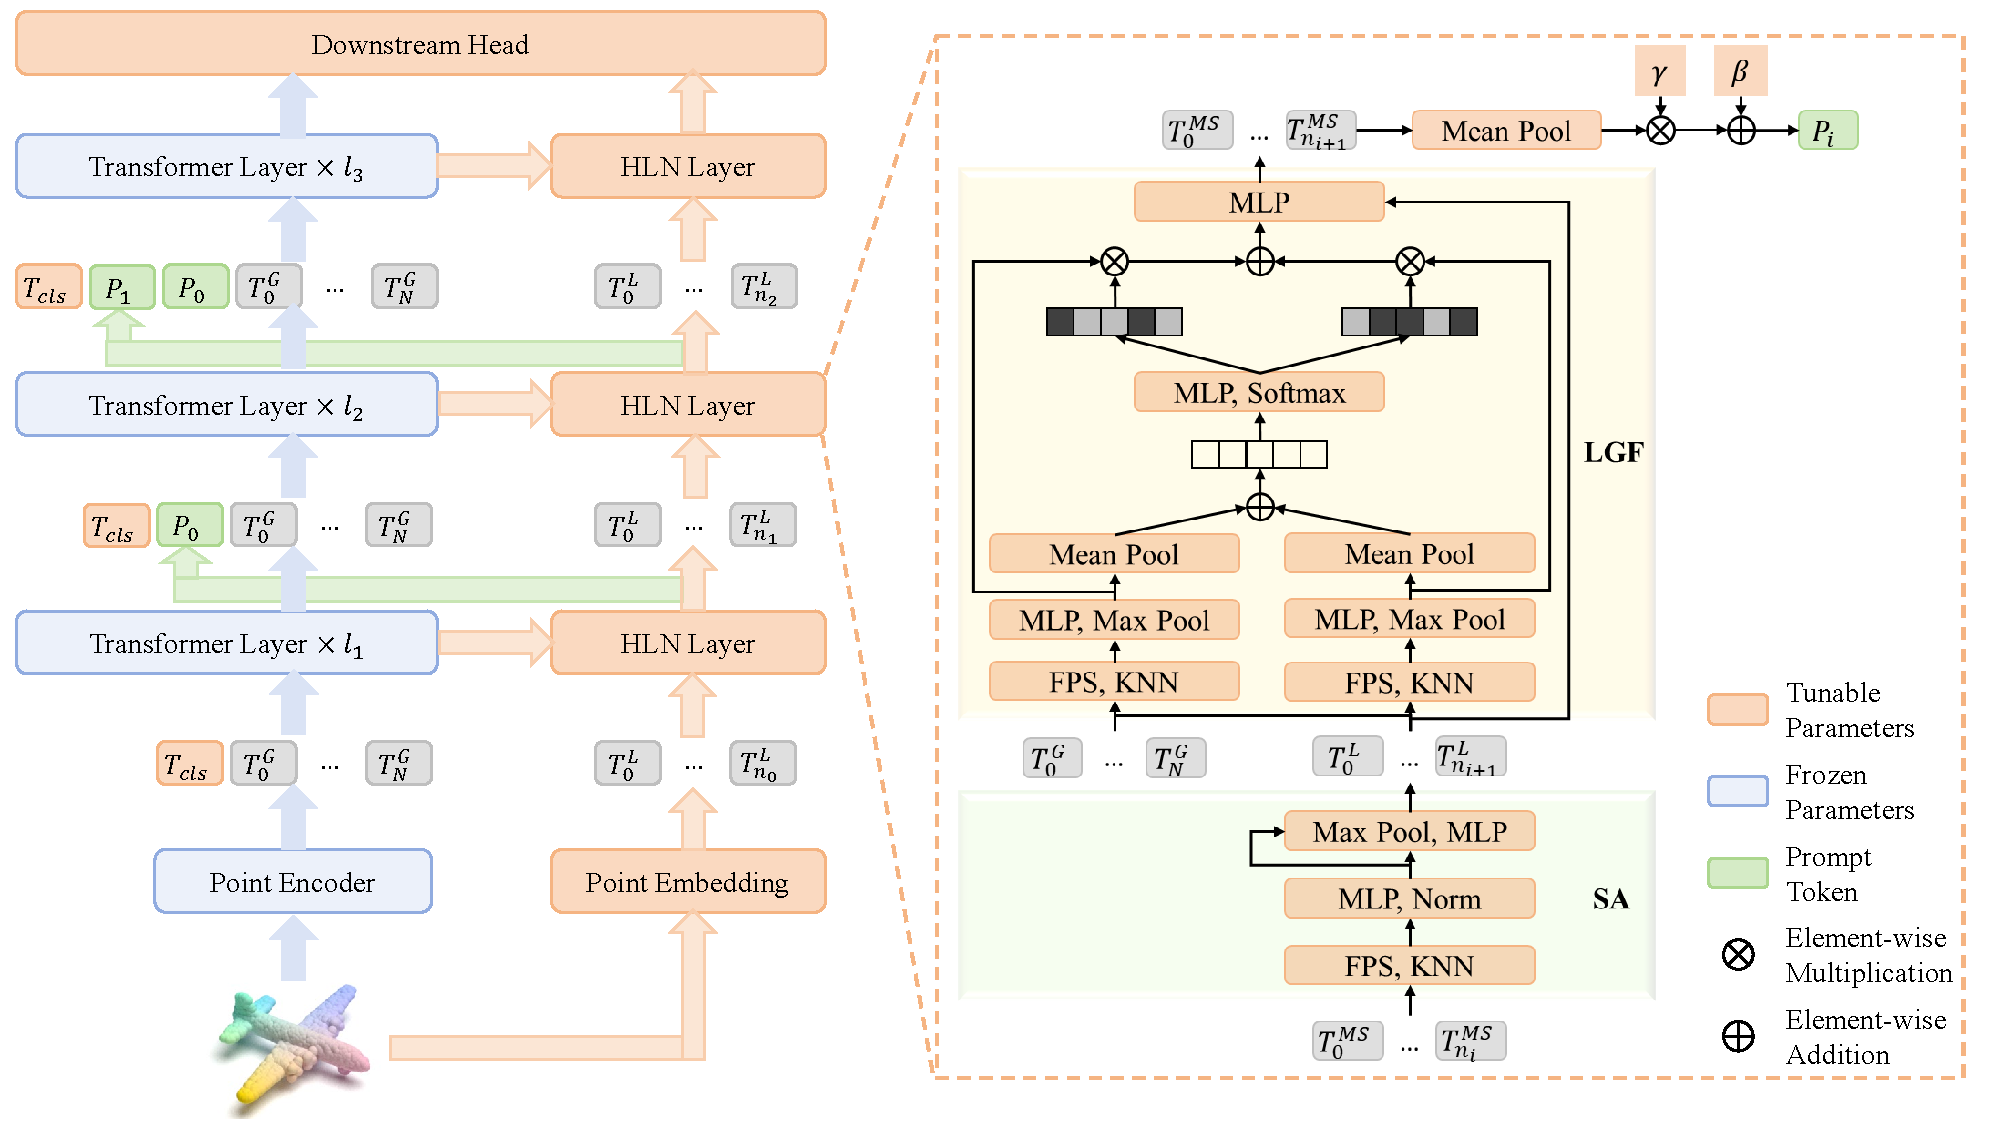
\includegraphics[width=\linewidth]{fig/Overall.pdf}
    \caption{The overall of our PLT. During fine-tuning, we froze the pre-trained backbone network and only fine-tune the PLT branch and the class token. The PLT branch consists of two main components: 1) Set Abstraction (SA), and 2) Local-Global Fusion Module (LGF).
}
    \label{fig:overall}
\end{figure*}

\section{Methodology}
\label{sec:methodology}

%To enable effective point cloud fine-tuning of pre-trained models while mitigating the high computational and storage costs associated with full-parameter updates, we propose Point Ladder Tuning (PLT), a parameter-efficient fine-tuning framework for 3D point cloud learning that that integrates hierarchically structured local pathways with dynamic multi-scale prompt guidance. PLT enhances parameter efficiency and task performance by jointly leveraging local geometric details and global semantic cues, thereby overcoming two key limitations: (1) the inability of Ladder Side-Tuning (LST)~\cite{sung2022lst} to effectively capture fine-grained local features, and (2) the limited instance-level adaptability of conventional prompt tuning methods~\cite{li2021prefix}.

We propose Point Ladder Tuning (PLT), an efficient method for fine-tuning pre-trained models on point clouds. PLT integrates hierarchical local pathways with multi-scale prompts, enhancing performance by combining local geometry with global semantics. PLT overcomes two drawbacks: (1) Ladder Side-Tuning’s difficulty capturing fine local details, and (2) standard prompt tuning’s weak instance-level adaptation.

As shown in Fig.~\ref{fig:overall2}, the core idea behind PLT is to decouple the fine-tuning process into two synergistic pathways: (1) a lightweight \textbf{Hierarchical Ladder Network (HLN)} that enriches task-specific local geometry modeling(\S\ref{sec:HLN}), and (2) a \textbf{Prompt-based Global Adaption} that dynamically modulates the frozen backbone via instance-aware multi-scale semantics(\S\ref{sec:FT_backbone}). These pathways are seamlessly integrated through a \textbf{Local-Global Fusion (LGF)} module that enables adaptive, bidirectional information exchange between local and global representations(\S\ref{sec:LGF}).

Finally, we design lightweight, task-specific heads, as detailed in \S\ref{sec:head}. Furthermore, we leverage the hierarchical structure to perform progressive upsampling, which facilitates the recovery of spatial resolution. This design choice proves especially effective for dense prediction tasks, where preserving spatial fidelity is crucial for accurate prediction.

\subsection{Hierarchical Ladder Network}
\label{sec:HLN}

%While transformer-based point cloud encoders excel at capturing global semantics, they often struggle with fine-grained spatial understanding due to their limited inductive bias toward local geometric structures. Existing PEFT methods (e.g. PointPEFT~\cite{tang2024point}, PointGST~\cite{liang2024parameter}) attempt to address this by introducing locality-enhancing modules, but still rely heavily on global activations from frozen backbones and typically operate at fixed resolutions, underutilizing the rich local context essential for dense prediction.

While transformer-based point cloud encoders capture global semantics well, they often miss fine-grained spatial details due to weak local geometric biases. Existing PEFT methods (e.g., PointPEFT, PointGST) try to improve locality but still depend heavily on frozen backbone features and fixed resolutions, missing key local details needed for dense prediction.

To solve this, we propose a Hierarchical Ladder Network (HLN) that extracts multi-resolution local features from point clouds. HLN better preserves 3D geometric structure, boosting performance in tasks like segmentation. It has two main components: (1) a Set Abstraction (SA) module (described here) and (2) a Local-Global Fusion (LGF) module.
% (detailed in Sec. ~\ref{sec:LGF}).

%To address these limitations, we propose a Hierarchical Ladder Network (HLN) to capture local information across multiple resolutions within the input point cloud. By explicitly modeling multi-scale local features, HLN better aligns with the geometric nature of 3D data and improves performance on tasks such as semantic segmentation. The HLN layer consists of two key components: (1) Set Abstraction (SA) and (2) Local-Global Fusion (LGF) module. In this section, we introduce SA, with LGF discussed further in Sec.~\ref{sec:LGF}.

Given an input point cloud $\mathbf{P} \in \mathbb{R}^{N \times 3}$, where $N$ is the number of points, we first apply point embedding to map $\mathbf{P}$ into a high-dimensional space, resulting in a initial point cloud features $\mathbf{F} \in \mathbb{R}^{N \times C}$, where $C$ represents the feature dimension. We then use Set Abstraction (SA) for downsampling, starting with farthest point sampling (FPS) to select a set of center points $\mathbf{C}=\{c_1, \ldots, c_n\}$, followed by k-Nearest Neighbors (kNN) to define local neighborhoods: 

\begin{equation}
    \mathcal{N}(c_i) = \left\{(\mathbf{p}_{c_i}^j, \mathbf{f}_{c_i}^j) \mid j = 1, \dots, k \right\}.
\end{equation}

The local features are aggregated as:
\begin{align}
    \hat{\mathbf{f}}_{c_i}^{j} &= \varphi\left(\left[\mathbf{f}_{c_i}^{j}; (\mathbf{p}_{c_i} - \mathbf{p}_{c_i}^j)\right]\right), \\
    \mathbf{f}_{c_i}^{\prime} &= \mathbf{f}_{c_i} + \rho\left(h_{\boldsymbol{\Theta}}([\hat{\mathbf{f}}_{c_i}^{1}; \dots; \hat{\mathbf{f}}_{c_i}^{k}])\right),
\end{align}
where $\varphi$, $\rho$ are learnable functions, $h_{\boldsymbol{\Theta}}$ denotes the aggregation function (e.g., max pooling) and $[\cdot ; \cdot]$ denotes concatenation. By stacking multiple SA layers, HLN constructs a hierarchical local representation $\mathbf{F}_l$ that complements global transformer outputs.

\subsection{Local-Global Fusion Module}
\label{sec:LGF}

A key challenge in point cloud representation learning is to effectively integrate fine-grained geometric details with high-level semantic context.. Existing fusion approaches, such as naive concatenation or element-wise addition, typically fail to adaptively balance these two information sources, leading to suboptimal performance, particularly in dense prediction tasks.

To address this issue, we propose a novel Local-Global Fusion (LGF) module that performs adaptive feature integration via selective attention. Our design is motivated by two key insights: (1) local geometric features extracted by the HLN pathway are critical for precise spatial reasoning; and (2) global features from the frozen pre-trained backbone encode rich semantic priors. LGF allows the network to dynamically balance and selectively integrate these complementary representations in a content-aware manner, ensuring that both local details and global semantics are effectively leveraged.

Let $\mathbf{F}_l$ and $\mathbf{F}_g$ denote local and global token features from HLN and the frozen backbone, respectively. we first map the backbone features to match the dimensionality of the HLN layer’s feature vectors using a learnable matrix $W$:

\begin{equation}
	\mathbf{F}_g' = \mathbf{F}_g W
\end{equation}

We then apply an aggregation operation similar to SA without spatial downsampling to capture cross-level interactions. This results in global features $\mathbf{F}_g''$, which model interactions between the local tokens $\mathbf{T}^{L}$ and global tokens $\mathbf{T}^{G}$, while $\mathbf{F}_l$ preserves the intra-local interactions within $\mathbf{T}^{L}$.

To fuse these global and local features, we employ a selective attention mechanism. This mechanism allows the model to focus adaptively on the most relevant information from each feature source, ensuring both global context and local details are integrated effectively. First, we apply an aggregation function $\mathcal{A}$, typically average pooling, to obtain global and local feature descriptors:

\begin{equation}
	\mathbf{f}_l = \mathcal{A}(\mathbf{F}_l), \quad \mathbf{f}_g = \mathcal{A}(\mathbf{F}_g'')
\end{equation}

These local and global descriptors are passed through an MLP to produce attention logits $\mathbf{z}_l$ and $\mathbf{z}_g$:
\begin{equation}
	\mathbf{z}_l, \mathbf{z}_g = \operatorname{split}\left( \alpha \left( \mathbf{f}_l + \mathbf{f}_g \right) \right)
\end{equation}
where $\alpha$ represents an MLP, $\operatorname{split}$ represents the splitting operation along the channel dimension.

We compute soft attention weights for both feature types using a softmax-like formulation:
\begin{equation}
	\mathbf{s}_l^i = \frac{e^{\mathbf{z}_l^i}}{e^{\mathbf{z}_l^i} + e^{\mathbf{z}_g^i}}, \quad
\mathbf{s}_g^i = \frac{e^{\mathbf{z}_g^i}}{e^{\mathbf{z}_l^i} + e^{\mathbf{z}_g^i}}.
\end{equation}

These weights are then used to obtain the fused multi-scale feature representation as a weighted sum:
\begin{equation}
	\mathbf{F}_{ms} = s_l \cdot \mathbf{F}_l + s_g \cdot \mathbf{F}_g''
\end{equation}

Finally, a lightweight MLP $\tau$ is applied to transform the fused features, and a residual connection adds this output to the shortcut features, producing the final fused output:
\begin{equation}
	\mathbf{F}_o = \mathbf{F}_l + \tau(\mathbf{F}_{ms})
\end{equation}

% By dynamically balancing the contributions of local and global representations, the LGF module enables effective integration of fine-grained geometry and high-level semantics. This fusion is especially beneficial for dense prediction tasks, where both local detail and global structure are critical to performance.

\subsection{Dynamic Prompt-Based Tuning}
\label{sec:FT_backbone}
To enable the pre-trained backbone network to produce task-adaptive global representations, we propose a dynamic multi-scale prompt generation strategy driven by the fused feature representation $\mathbf{F}_{o}$ from the LGF module. This design aims to inject instance-specific geometric cues into the transformer backbone, allowing the model to preserve general semantic priors while adapting flexibly to downstream tasks.

Firstly, $F_{o}$ is mean-pooled to obtain a compact representation. This pooled feature is then scaled and shifted using learnable parameters $\gamma$ and $\beta$, generating a multi-scale prompt $\mathbf{p}$. To maximize parameter efficiency, we reuse $W$ from the LGF module to align the dimensionality of the multi-scale prompts with that of the backbone network features. The formula for this process is as follows:
\begin{equation}
	\mathbf{p} = \left(\gamma \cdot \frac{1}{n} \sum_{i=1}^{n} \mathbf{F}_o^i + \beta \right) W^T
\end{equation}
where $n$ is the number of tokens in $F_o$.

Finally, the multi-scale prompts $\mathbf{P}=[\mathbf{p}_{1}, \ldots, \mathbf{p}_{s}]$ are incorporated into the backbone network during training, where $s$ is corresponds to the number of stages in the HLN pathway. These prompts are inserted at each transformer layer of the frozen backbone to condition the global representation in a scale-aware, instance-sensitive manner:
\begin{equation}
	\mathbf{x}_l = \mathcal{L}_l\left([\mathbf{T}_{cls}; \mathbf{P}; \mathbf{T}^{G}]\right)
\end{equation}
where $\mathcal{L}_l$ is the $l$-th transformer layer. 

The injected prompts participate in the attention mechanism, interacting with the original tokens to enrich the contextual modeling without altering the backbone’s architecture. This allows the model to adaptively refine global features based on the special task, while maintaining the semantic richness of large-scale pre-training.

To further enhance adaptability, we adopt the lightweight scale-and-shift tuning strategy proposed in SSF~\cite{lian2022scaling}, applying element-wise affine transformations to the output of each backbone module:

\begin{equation}
	\mathbf{y} = s \cdot \mathbf{x} + t
\end{equation}
where $s$ and $t$ are learnable  scaling and shifting  vectors that fine-tune the global representation with minimal overhead.

Our dynamic prompt-based tuning mechanism combines geometry-aware conditioning with parameter-efficient tuning (PEFT) to enable flexible and effective adaptation to diverse 3D tasks, without requiring task-specific adapters or modifying the backbone. This design significantly increases model expressiveness and task-specific responsiveness, while preserving efficiency and scalability.

\subsection{Downstream Head}
\label{sec:head}

\subsubsection{Classification Head}
For classification tasks, we aggregate local-global cues into a compact descriptor as follows:

\begin{equation}
\mathbf{x}_o = [\mathbf{T}_{cls} + \mathcal{A}_{\text{avg}}(\mathbf{P}); \mathcal{A}_{\text{max}}(\mathbf{T}^{G}); \mathcal{A}_{\text{max}}(\mathbf{T}^{L})]
\end{equation}
where $\mathcal{A}_{\text{avg}}$ and $\mathcal{A}_{\text{max}}$ denote average pooling and max pooling operations, respectively. This aggregated descriptor is then fed into a MLP, followed by a softmax activation to produce the final classification output:
\begin{equation}
\mathbf{y}_{cls} = \operatorname{softmax}(\operatorname{MLP}(\mathbf{x}_o))
\label{eq:MLP}
\end{equation}


\subsubsection{Segmentation Head}
Unlike classification tasks, semantic segmentation requires per-point predictions, necessitating the recovery of features for all original points. A common approach is to propagate features from downsampled representations back to the original point cloud through feature interpolation. However, most existing parameter-efficient fine-tuning methods~\cite{zha2023instance,zhou2024dynamic,liang2024parameter} for point cloud lack the ability to capture multi-resolution information, leading to a considerable loss of local detail.

To address this issue, we introduce an additional HLN branch to extract fine-grained multi-resolution features from the spatial domain. Inspired by PointNext~\cite{qian2022pointnext}, we employ an inverse distance-weighted interpolation strategy to progressively recover the point-level features at each resolution. Different from PointNext~\cite{qian2022pointnext}, we simultaneously leverage both the global features from the backbone and the multi-resolution local features from HLN to upsample. During each interpolation step, these are concatenated to form a comprehensive representation:

\begin{equation}
\mathbf{T}^{\text{interp}} = [\operatorname{Interp}(\mathbf{T}, \mathbf{T}^G); \operatorname{Interp}(\mathbf{T}, \mathbf{T}^L)]
\end{equation}
where $\mathbf{T}$ denotes the point features at the current layer. The function $\operatorname{Interp}(\cdot)$ performs inverse distance interpolation~\cite{qian2022pointnext}.

At each resolution, we concatenate the interpolated features $\mathbf{T}^{\text{interp}}$ with the corresponding original features $\mathbf{T}$, and then pass them through a MLP to obtain updated features. This process is repeated iteratively until the resolution of the original point cloud is restored. Finally, point-wise classification is performed using a MLP followed by a softmax activation, as defined in Eq.~\eqref{eq:MLP}, to predict the semantic category of each point. This design not only enhances segmentation performance but also substantially reduces the number of trainable parameters and overall computational complexity.

